% NOTES:
% (DONE)
%   Take more time to justify why decentralized environments, the use-case is good but:
%       - Mention how its only one of the use-cases (check)
%       - Explain it more how decentralized matters with more anecdotes (check)
%       - Transition from centralized to link traversal doesn't make any goddamn sense (check)
%       - Why do we use documents? Why not sparql endpoints? Documents are very unexpressive allowing flexible data representation without large server cost.
%       - User in the loop privacy controls instead of granular, once data is in centralized storage its difficult to get it out.
%       - Maybe remove the slide talking about centralized querying
%       - Document serving of resources is less expressive (can answer less types of questions, just what is in the document)
%         becomes less expensive per level of granularity fine-grained access control

\begin{frame}{The Need for Decentralized Personal Data Storage}
    \begin{columns}[T] % T aligns columns at the top
        % Left column: Image
        \begin{column}{0.6\textwidth} % Adjust width as needed
            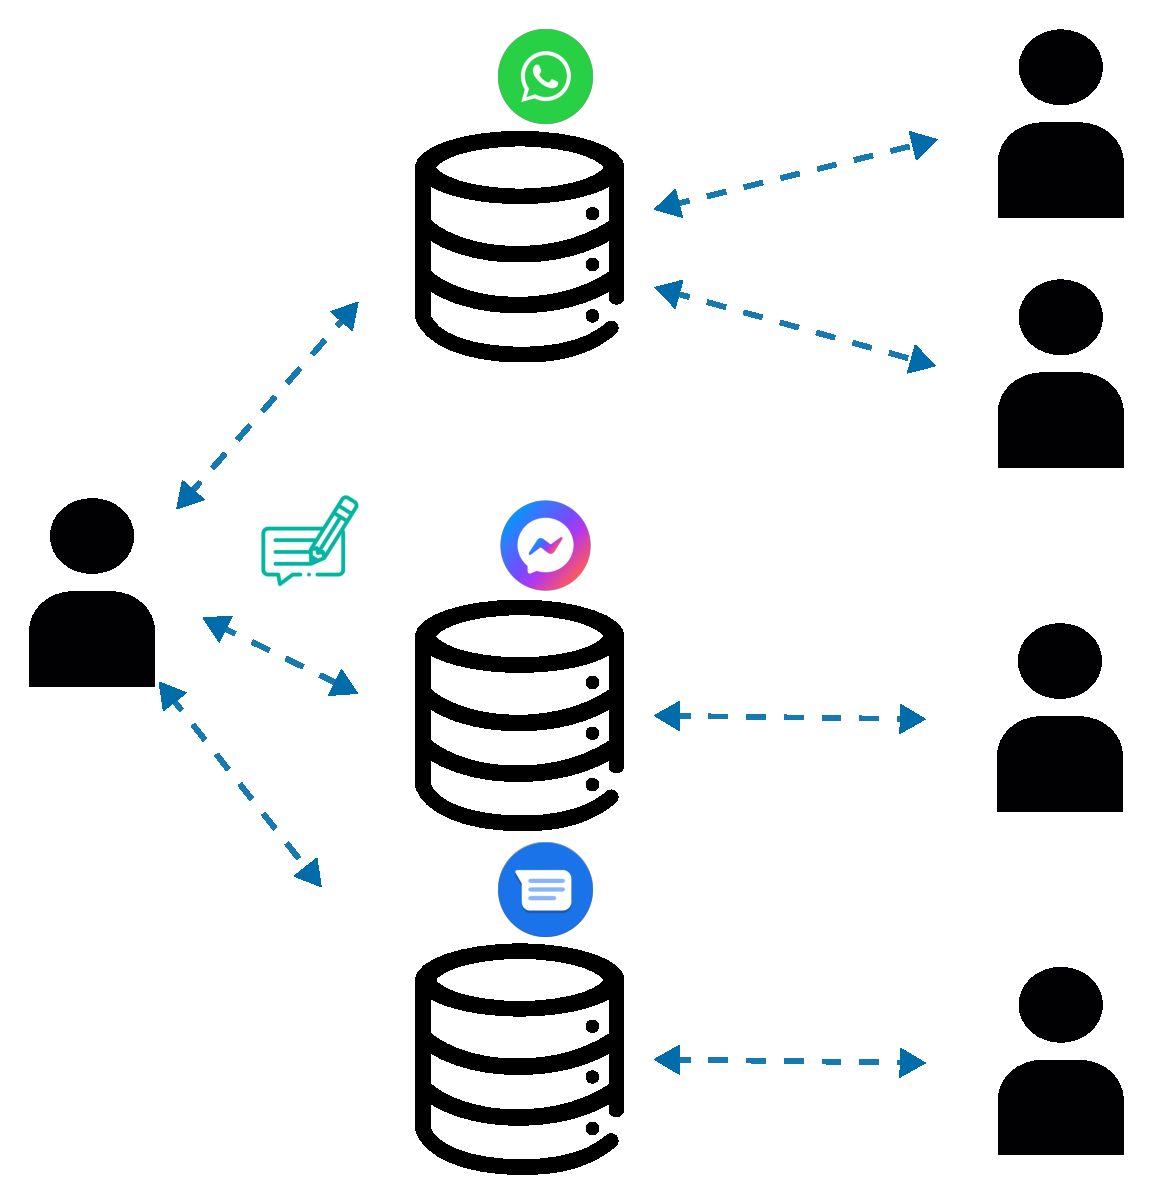
\includegraphics[width=.85\linewidth]{images/current-bad-message-situation.pdf} % replace with your image file
        \end{column}

        % Right column: Text
        \begin{column}{0.4\textwidth} % Adjust width as needed
            \begin{itemize}
                \item Each application has its own data
                \item Stifles innovation
                \item Causes vendor lock-in
            \end{itemize}
        \end{column}
    \end{columns}
\end{frame}


\begin{frame}{The Need for Decentralized Personal Data Storage}
    \begin{columns}[T] % T aligns columns at the top
        % Left column: Image
        \begin{column}{0.6\textwidth} % Adjust width as needed
            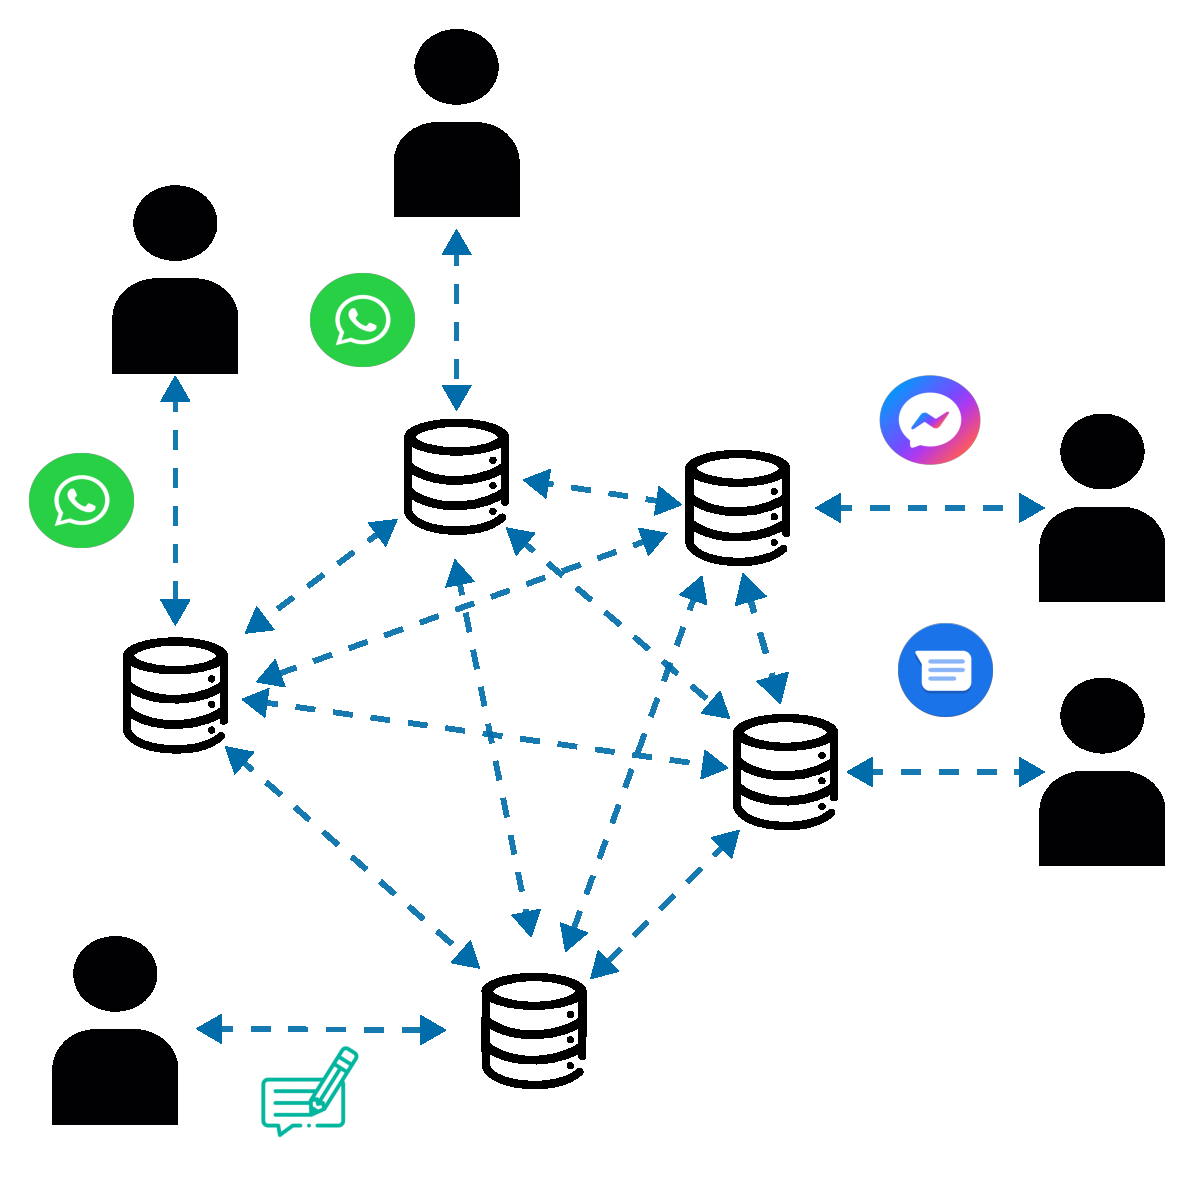
\includegraphics[width=.9\linewidth]{images/decentralized-message-storage.pdf} % replace with your image file
        \end{column}

        % Right column: Text
        \begin{column}{0.4\textwidth} % Adjust width as needed
            \begin{itemize}
                \item Each application uses common data storage
                \item Easy to switch vendors
                \item Promotes innovation
            \end{itemize}
        \end{column}
    \end{columns}
\end{frame}

\begin{frame}{The Problem with Centrally Aggregating and Querying}
    \begin{columns}[T] % T aligns columns at the top
        % Left column: Image
        \begin{column}{0.6\textwidth} % Adjust width as needed
            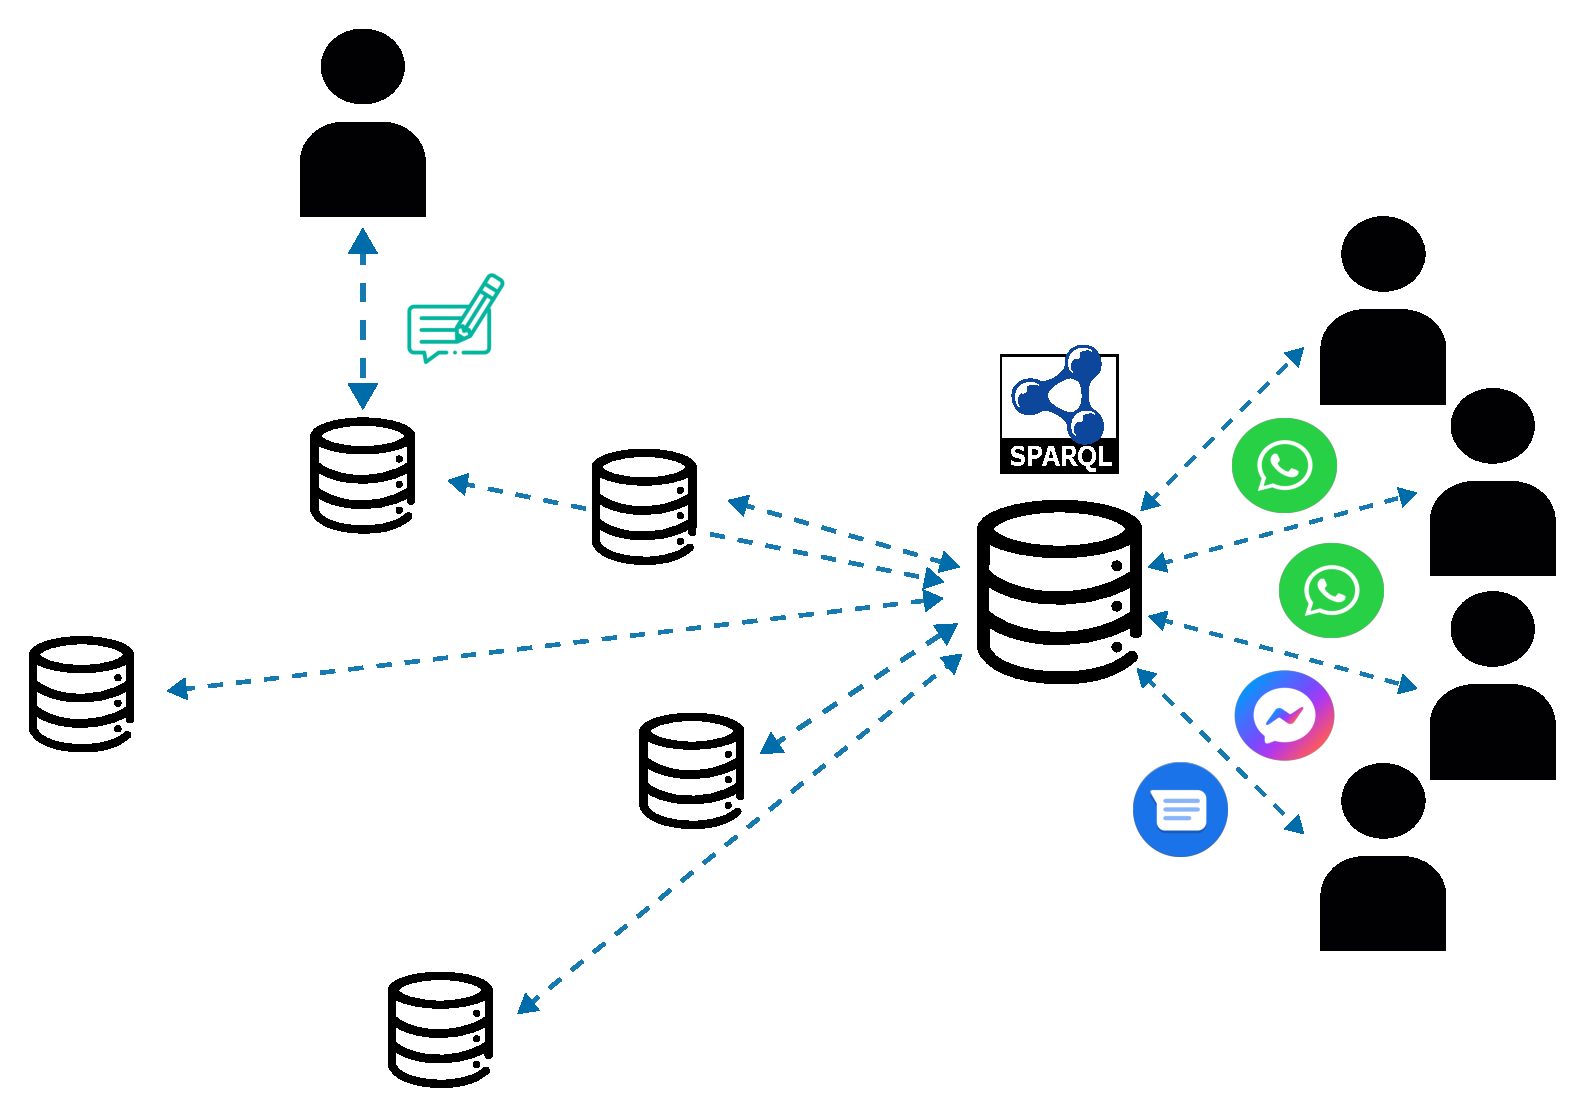
\includegraphics[width=\linewidth]{images/centralize-personal-data-stores.pdf} % replace with your image file
        \end{column}

        % Right column: Text
        \begin{column}{0.4\textwidth} % Adjust width as needed
            \begin{itemize}
                \item Why not aggregate data and query it?
                \item Difficult in case of personal data due to privacy concerns
            \end{itemize}
        \end{column}
    \end{columns}
\end{frame}

\begin{frame}{The Problem with Centrally Aggregating and Querying}
    \begin{columns}[T] % T aligns columns at the top
        % Left column: Image
        \begin{column}{0.6\textwidth} % Adjust width as needed
            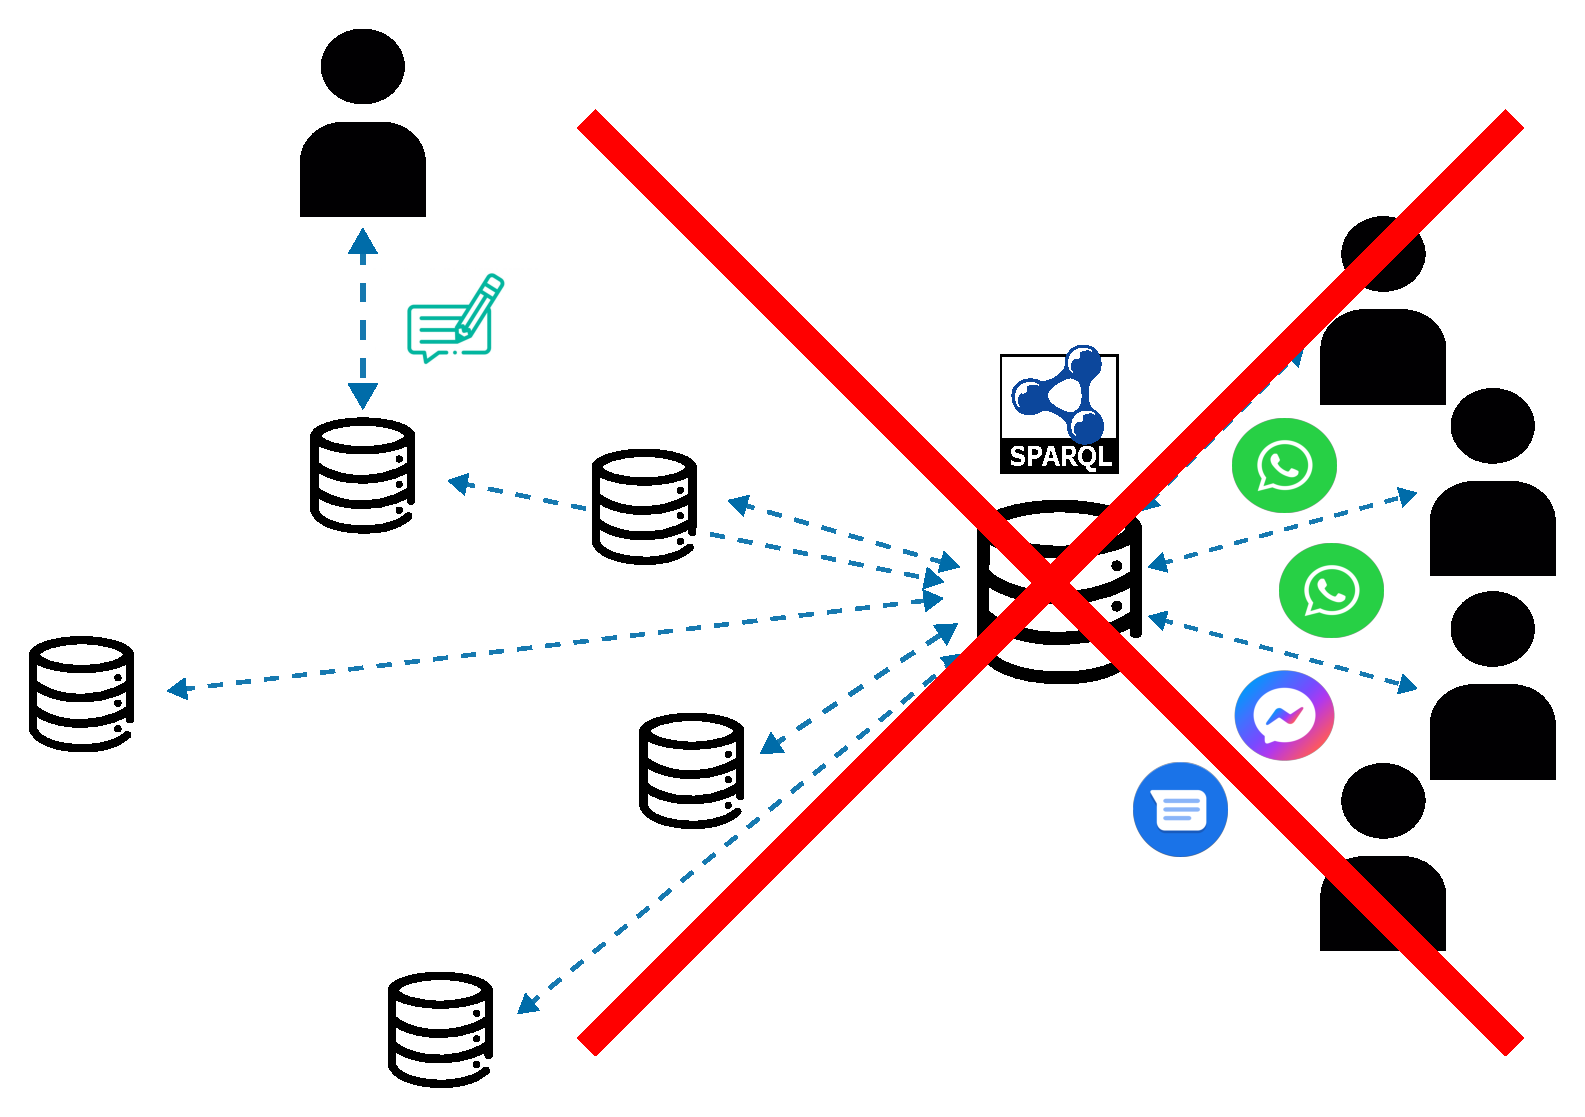
\includegraphics[width=\linewidth]{images/centralize-personal-data-stores-no.pdf} % replace with your image file
        \end{column}

        % Right column: Text
        \begin{column}{0.4\textwidth} % Adjust width as needed
            \begin{itemize}
                \item Why not aggregate data and query it?
                \item Difficult in case of personal data due to privacy concerns
            \end{itemize}
        \end{column}
    \end{columns}
\end{frame}

